\documentclass[varwidth=7.7cm]{standalone}
\usepackage{pgfplots}
\pgfplotsset{compat=1.18} % Ensure compatibility with the specified version
\usepgfplotslibrary{statistics}
\usepgflibrary{plotmarks}
\usetikzlibrary{calc, patterns}

\usepackage{xcolor}
\usepackage{pifont}
\newcommand{\cmark}{\ding{51}}  
\newcommand{\xmark}{\ding{55}}

\definecolor{ibm1}{HTML}{0077BB}
\definecolor{ibm2}{HTML}{33BBEE}
\definecolor{ibm3}{HTML}{EE7733}
\definecolor{ibm4}{HTML}{EE3377}
\definecolor{ibm5}{HTML}{CC3311}

\definecolor{grad1}{HTML}{364B9A}
\definecolor{grad2}{HTML}{98CAE1}
\definecolor{grad3}{HTML}{FEDA8B}
\definecolor{grad4}{HTML}{DD3D2D}
\definecolor{grad5}{HTML}{A50026}

\begin{document}

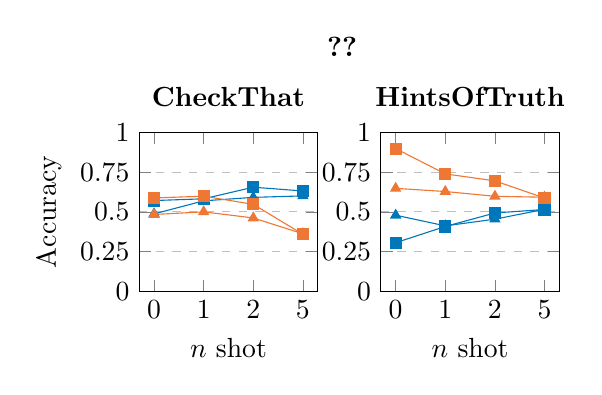
\begin{tikzpicture}
    \begin{axis}[
        title={\textbf{CheckThat}},
        name={ct},
        xlabel={$n$ shot},
        ylabel={Accuracy},
        width=3.85cm,
        height=3.6cm,
        ymin=0, ymax=1,
        ytick={0,0.25,0.5,0.75,1},
        legend to name={legend-icl-perf},
        legend style={
            draw=none,
            fill=none,
        },
        legend columns=2, 
        xtick=data,
        ymajorgrids=true,
        grid style=dashed,
        symbolic x coords={0, 1, 2, 5}, 
    ]

    \addplot[
        color=ibm1,
        mark=square*,
    ]
    coordinates {
(0, 0.5711678832116789)
(1, 0.5821167883211679)
(2, 0.6551094890510949)
(5, 0.6313868613138686)
    };
    \addlegendentry{Llava, short}

    \addplot[
        color=ibm1,
        mark=triangle*,
    ]
    coordinates {
(0, 0.48722627737226276)
(1, 0.5693430656934306)
(2, 0.5912408759124088)
(5, 0.6003649635036497)
    };
    \addlegendentry{Llava, long}

    \addplot[
        color=ibm3,
        mark=square*,
    ]
    coordinates {
(0, 0.5875912408759124)
(1, 0.5985401459854015)
(2, 0.5474452554744526)
(5, 0.359)
    };
    \addlegendentry{Pixtral, short}

    \addplot[
        color=ibm3,
        mark=triangle*,
    ]
    coordinates {
(0, 0.4835766423357664)
(1, 0.5)
(2, 0.46167883211678834)
(5, 0.362)
    };
    \addlegendentry{Pixtral, long}
    \end{axis}

    \begin{axis}[
        at={($(ct.east)+(.8cm, 0)$)},
        name={ob},
        anchor=west,
        title={\textsc{\textbf{HintsOfTruth}}},
        xlabel={$n$ shot},
        width=3.85cm,
        height=3.6cm,
        ytick={0,0.25,0.5,0.75,1},
        ymin=0, ymax=1,
        legend pos=north west,
        xtick=data,
        ymajorgrids=true,
        grid style=dashed,
        symbolic x coords={0, 1, 2, 5}, 
    ]

    \addplot[
        color=ibm1,
        mark=square*,
    ]
    % llava short
    coordinates {
(0,0.306)
(1,0.408)
(2,0.493)
(5,0.515)
    };
    \addplot[
        color=ibm1,
        mark=triangle*,
    ]
    % llava long
    coordinates {
(0,0.479)
(1,0.412)
(2,0.454)
(5,0.516)
    };
    \addplot[
        color=ibm3,
        mark=square*,
    ]
    % pixtral short
    coordinates {
(0,0.898)
(1,0.739)
(2,0.695)
(5,0.587)
    };
    \addplot[
        color=ibm3,
        mark=triangle*,
    ]
    % pixtral long
    coordinates {
(0,0.648)
(1,0.628)
(2,0.598)
(5,0.592)
    };
    \end{axis}
    \node at ($(ct.east)!0.5!(ct.east)+(.31cm, 2.1)$) {\ref{legend-icl-perf}};
\end{tikzpicture}

\end{document}
